\documentclass[xetex,mathserif,serif,handout]{beamer}

\usepackage{xunicode}
\usepackage{xltxtra}
\usepackage{color}
\usepackage{url}
\usepackage{listings}
\usepackage{fontspec}
\usepackage{geometry}
\usepackage{lastpage}
\usepackage{fancyhdr}
\usepackage{amsmath}
\usepackage{amsthm}
\usepackage{amssymb}
\usepackage{blkarray}
\usepackage{multicol}
\usepackage{relsize}

\definecolor{solarized@base03}{HTML}{002B36}
\definecolor{solarized@base02}{HTML}{073642}
\definecolor{solarized@base01}{HTML}{586e75}
\definecolor{solarized@base00}{HTML}{657b83}
\definecolor{solarized@base0}{HTML}{839496}
\definecolor{solarized@base1}{HTML}{93a1a1}
\definecolor{solarized@base2}{HTML}{EEE8D5}
\definecolor{solarized@base3}{HTML}{FDF6E3}
\definecolor{solarized@yellow}{HTML}{B58900}
\definecolor{solarized@orange}{HTML}{CB4B16}
\definecolor{solarized@red}{HTML}{DC322F}
\definecolor{solarized@magenta}{HTML}{D33682}
\definecolor{solarized@violet}{HTML}{6C71C4}
\definecolor{solarized@blue}{HTML}{268BD2}
\definecolor{solarized@cyan}{HTML}{2AA198}
\definecolor{solarized@green}{HTML}{859900}
\definecolor{yaleblue}{HTML}{0E4C92}

\setbeamertemplate{navigation symbols}{}
% \setbeamerfont{title}{family=\old}
% \setbeamerfont{author}{family=\tfont}%
% \setbeamerfont{frametitle}{family=\oldA}
% \setbeamerfont{date}{family=\dfont}

\setbeamertemplate{itemize items}{--}
\setbeamercolor*{item}{fg=black}

\defaultfontfeatures{Mapping=tex-text}
\hypersetup{pdfstartview={FitH}}

\newcommand{\old}[1]{\fontspec[Alternate=1,Ligatures={Common}]{Hoefler Text}\fontsize{18pt}{30pt}\selectfont #1}%
\newcommand{\oldA}[1]{\fontspec[Alternate=1,Ligatures={Common, Rare}]{Hoefler Text}\fontsize{12pt}{15pt}\selectfont #1}%
\newcommand{\oldB}[1]{\fontspec[Ligatures={Common}]{Didot}\fontsize{12pt}{15pt}\color{solarized@base02}\selectfont #1}%
\newcommand{\tfont}[1]{\fontspec[Alternate=1,Ligatures={Common}]{Hoefler Text}\fontsize{12pt}{20pt}\selectfont #1}%
\newcommand{\dfont}[1]{\fontspec[Ligatures={Common}]{Didot}\fontsize{12pt}{12pt}\selectfont #1}%

\newcommand{\minimize}{\mathop{\mathrm{minimize}}}
\newcommand{\argmin}{\mathop{\mathrm{arg\,min}}}
\newcommand{\argmax}{\mathop{\mathrm{arg\,max}}}
\newcommand{\st}{\mathop{\mathrm{subject\,\,to}}}

\newcommand\independent{\protect\mathpalette{\protect\independenT}{\perp}}
\def\independenT#1#2{\mathrel{\rlap{$#1#2$}\mkern2mu{#1#2}}}

\setlength{\parindent}{0pt}
\setlength{\parskip}{12pt}

\setromanfont [Ligatures={Common}, Numbers={OldStyle}, Variant=01,
 BoldFont={LinLibertine_RB.otf},
 ItalicFont={LinLibertine_RI.otf},
 BoldItalicFont={LinLibertine_RBI.otf}
 ]{LinLibertine_R.otf}



\begin{document}

%%%%%%%%%%%%%%%%%%%%%%%%%%%%%%%%%%%%%%%%%%%%%%%%%%%
\begin{frame}[fragile] \frametitle{}

\vfill

{\fontsize{0.7cm}{0cm}\selectfont Lecture 14 \\\vspace{0.2cm}
Singular Value Decomposition}\\\vspace{0.5cm}
02 November 2015

\vspace{2cm}

\begin{minipage}{0.6\textwidth}
Taylor B. Arnold \\
Yale Statistics \\
STAT 312/612
\end{minipage}
\hfill
\begin{minipage}{0.3\textwidth}\raggedleft

\includegraphics[scale=0.3]{../yale-logo.png}
\end{minipage}%

\end{frame}

%%%%%%%%%%%%%%%%%%%%%%%%%%%%%%%%%%%%%%%%%%%%%%%%%%%
\begin{frame}[fragile] \frametitle{}

{\color{yaleblue}\fontsize{16pt}{20pt}\selectfont Goals for today}

\begin{itemize}
\item singular value decomposition
\item condition numbers
\item application to mean squared errors
\item (time permitting) image dataset
\end{itemize}

\end{frame}

%%%%%%%%%%%%%%%%%%%%%%%%%%%%%%%%%%%%%%%%%%%%%%%%%%%
\begin{frame}[fragile] \frametitle{}

A matrix $A \in \mathbb{R}^{n \times m}$ can be thought of as
a linear mapping between two spaces:
\begin{align*}
A: \mathbb{R}^m \rightarrow \mathbb{R}^n
\end{align*}
This interpretation requires no assumptions on the shape or
structure of the matrix $A$.

\end{frame}

%%%%%%%%%%%%%%%%%%%%%%%%%%%%%%%%%%%%%%%%%%%%%%%%%%%
\begin{frame}[fragile] \frametitle{}

The singular value decomposition writes the matrix $A$ as a product
of three matricies:
\begin{align*}
A &= U \Sigma V^t
\end{align*}
Where $U \in \mathbb{R}^{n\times n}$ and $V \in \mathbb{R}^{m\times m}$
are orthonormal matricies and $\Sigma$ is the rectangular diagonal matrix
$\text{diag}(\sigma_1, \sigma_2, \ldots, \sigma_{\text{min}(n,m)})$.

\pause This decompositon exists for any real matrix $A$.

\end{frame}

%%%%%%%%%%%%%%%%%%%%%%%%%%%%%%%%%%%%%%%%%%%%%%%%%%%
\begin{frame}[fragile] \frametitle{}

By convention, the values of $\Sigma$ are arranged in decending
order: $\sigma_1 \geq \sigma_2 \geq \cdots \geq \sigma_{\text{min}(n,m)}$.

\pause These are called the \textbf{singular values} of the matrix $A$.

\pause The number of non-zero singular values is equal to the rank of the
matrix $A$.

\end{frame}

%%%%%%%%%%%%%%%%%%%%%%%%%%%%%%%%%%%%%%%%%%%%%%%%%%%
\begin{frame}[fragile] \frametitle{}

The singular value decomposition allows us to write the matrix $A$ as a sum
of $r$, rank $1$ matricies:
\begin{align*}
A &= \sum_i^{r=\text{rank}(A)} \sigma_i u_i v_i^t
\end{align*}

\end{frame}

%%%%%%%%%%%%%%%%%%%%%%%%%%%%%%%%%%%%%%%%%%%%%%%%%%%
\begin{frame}[fragile] \frametitle{}

A useful way of viewing the singular value decomposition is to think about
what would happen when projecting columns of $U$ and $V$:
\begin{align*}
A v_i &= \sigma_i u_i \\
A^t u_i &= \sigma_i v_i
\end{align*}
\pause Notice that both equations use $\sigma_i$!

\end{frame}

%%%%%%%%%%%%%%%%%%%%%%%%%%%%%%%%%%%%%%%%%%%%%%%%%%%
\begin{frame}[fragile] \frametitle{}

Therefore, if we have an arbitrary vector $z \in \mathbb{R}^m$
and we write it in the basis of $V$:
\begin{align*}
z &= \sum_i \alpha_i v_i
\end{align*}
The mapping of $A$ can be easily calculated in the coordinate system
of $U$:
\begin{align*}
Az &= \sum_i \alpha_i \sigma_i u_i
\end{align*}
Due to the linearity of the matrix operation.

\end{frame}

%%%%%%%%%%%%%%%%%%%%%%%%%%%%%%%%%%%%%%%%%%%%%%%%%%%
\begin{frame}[fragile] \frametitle{}

\begin{center}
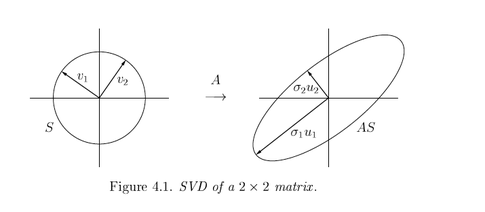
\includegraphics[width=\textwidth]{img/svd_2d.png}
\end{center}

\end{frame}


%%%%%%%%%%%%%%%%%%%%%%%%%%%%%%%%%%%%%%%%%%%%%%%%%%%
\begin{frame}[fragile] \frametitle{}

As an example, let's construct a $2$-by-$3$ matrix:

\begin{verbatim}
> A <- matrix(1:6,ncol=3)
> A
     [,1] [,2] [,3]
[1,]    1    3    5
[2,]    2    4    6
\end{verbatim}

\end{frame}

%%%%%%%%%%%%%%%%%%%%%%%%%%%%%%%%%%%%%%%%%%%%%%%%%%%
\begin{frame}[fragile] \frametitle{}

The singular value decomposition can be calculated by
the \texttt{svd} function in R. By default only $\text{min}(n,m)$
columns of $U$ and $V$ are calculated, but we'll ask for all
of them here.
\begin{verbatim}
> svd(A, nu=2, nv=3)
$d
[1] 9.5255181 0.5143006

$u
           [,1]       [,2]
[1,] -0.6196295 -0.7848945
[2,] -0.7848945  0.6196295

$v
           [,1]       [,2]       [,3]
[1,] -0.2298477  0.8834610  0.4082483
[2,] -0.5247448  0.2407825 -0.8164966
[3,] -0.8196419 -0.4018960  0.4082483
\end{verbatim}

\end{frame}

%%%%%%%%%%%%%%%%%%%%%%%%%%%%%%%%%%%%%%%%%%%%%%%%%%%
\begin{frame}[fragile] \frametitle{}

We can extract the three components of the SVD and
verify that the matrix $A$ is returned:
\begin{verbatim}
> SVD <- svd(A, nu=2, nv=3)
> Sigma <- cbind(diag(SVD$d),0)
> U <- SVD$u
> V <- SVD$v
> A - U %*% Sigma %*% t(V)
             [,1]         [,2] [,3]
[1,] 2.220446e-16 4.440892e-16    0
[2,] 0.000000e+00 4.440892e-16    0
\end{verbatim}
\pause Notice that there are some small errors in the decomposition.

\end{frame}

%%%%%%%%%%%%%%%%%%%%%%%%%%%%%%%%%%%%%%%%%%%%%%%%%%%
\begin{frame}[fragile] \frametitle{}

\begin{verbatim}
> N <- 1e5
> p <- 3
> unitBall <- matrix(runif(N * p, -1, 1), nrow=3)
> unitBall <- unitBall[,apply(unitBall^2, 2, sum) < 1]
> unitBall[,1:5]
          [,1]       [,2]       [,3]       [,4]        [,5]
[1,] 0.5287973 -0.7040859 -0.7248478 -0.4671987  0.05705657
[2,] 0.4255332 -0.3016897  0.3072752  0.5290554  0.78391679
[3,] 0.5349525 -0.4057218 -0.5348268 -0.3940231 -0.51866525
\end{verbatim}

\end{frame}

%%%%%%%%%%%%%%%%%%%%%%%%%%%%%%%%%%%%%%%%%%%%%%%%%%%
\begin{frame}[fragile] \frametitle{}

\begin{verbatim}
> projUnitBall <- t(A %*% unitBall)
> head(projUnitBall)
           [,1]       [,2]
[1,]  4.4801594  5.9694424
[2,] -3.6377640 -5.0492614
[3,] -2.4771562 -3.4295556
[4,] -0.8501476 -1.1823139
[5,] -0.1845193  0.1377888
[6,]  4.8409047  5.9547905
> plot(projUnitBall,pch=".")
\end{verbatim}

\end{frame}

%%%%%%%%%%%%%%%%%%%%%%%%%%%%%%%%%%%%%%%%%%%%%%%%%%%
\begin{frame}[fragile] \frametitle{}

\begin{center}
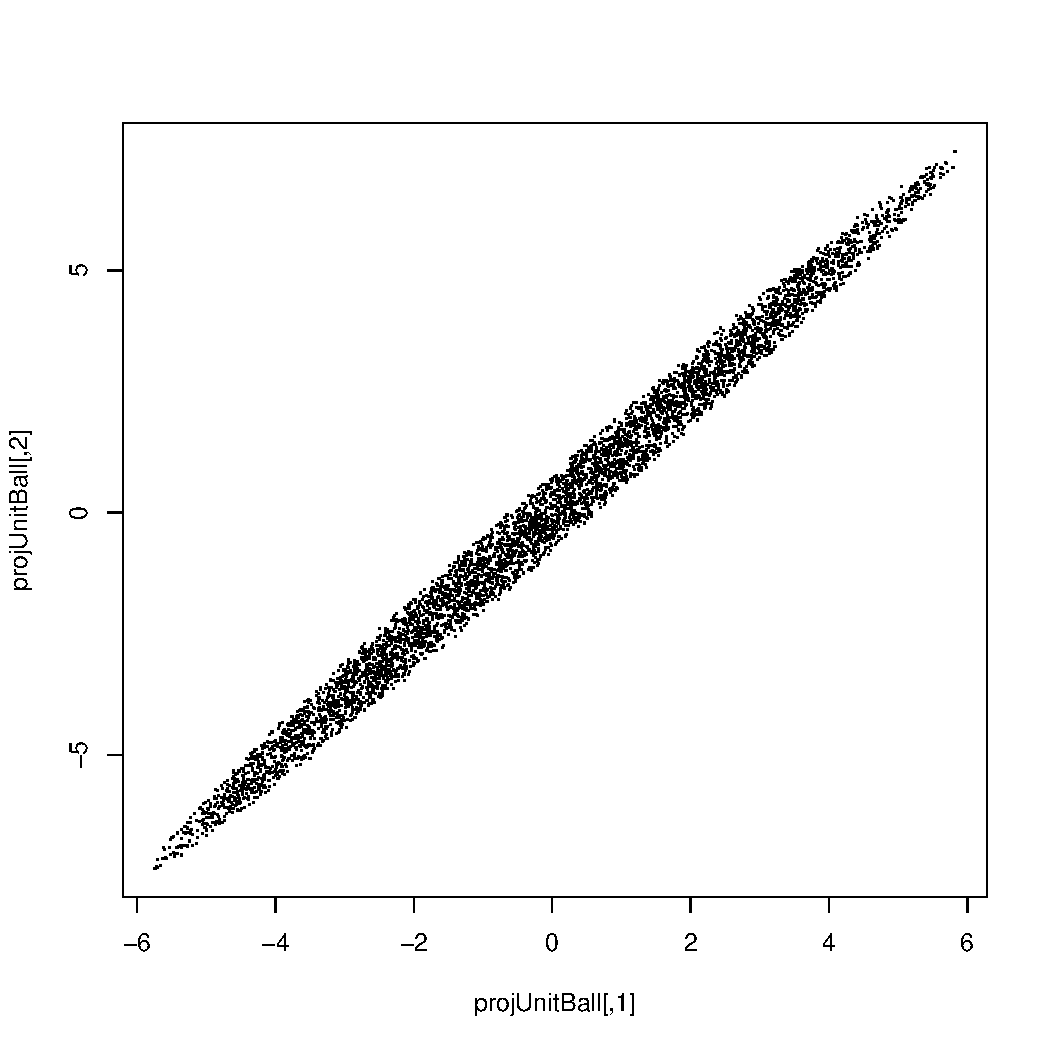
\includegraphics[width=3.5in]{img/fig04.pdf}
\end{center}

\end{frame}

%%%%%%%%%%%%%%%%%%%%%%%%%%%%%%%%%%%%%%%%%%%%%%%%%%%
\begin{frame}[fragile] \frametitle{}

\begin{verbatim}
> A %*% V
          [,1]       [,2]         [,3]
[1,] -5.902292 -0.4036717 8.881784e-16
[2,] -7.476526  0.3186758 4.440892e-16
> sqrt(apply((A %*% V)^2, 2, sum))
 [1] 9.525518e+00 5.143006e-01 9.930137e-16
>
> v1 <- (A %*% V)[,1]
> v2 <- (A %*% V)[,2]
> arrows(0,0,v1[1],v1[2],col="red",lwd=2)
> arrows(0,0,v2[1],v2[2],col="green",lwd=2)
\end{verbatim}

\end{frame}

%%%%%%%%%%%%%%%%%%%%%%%%%%%%%%%%%%%%%%%%%%%%%%%%%%%
\begin{frame}[fragile] \frametitle{}

\begin{center}
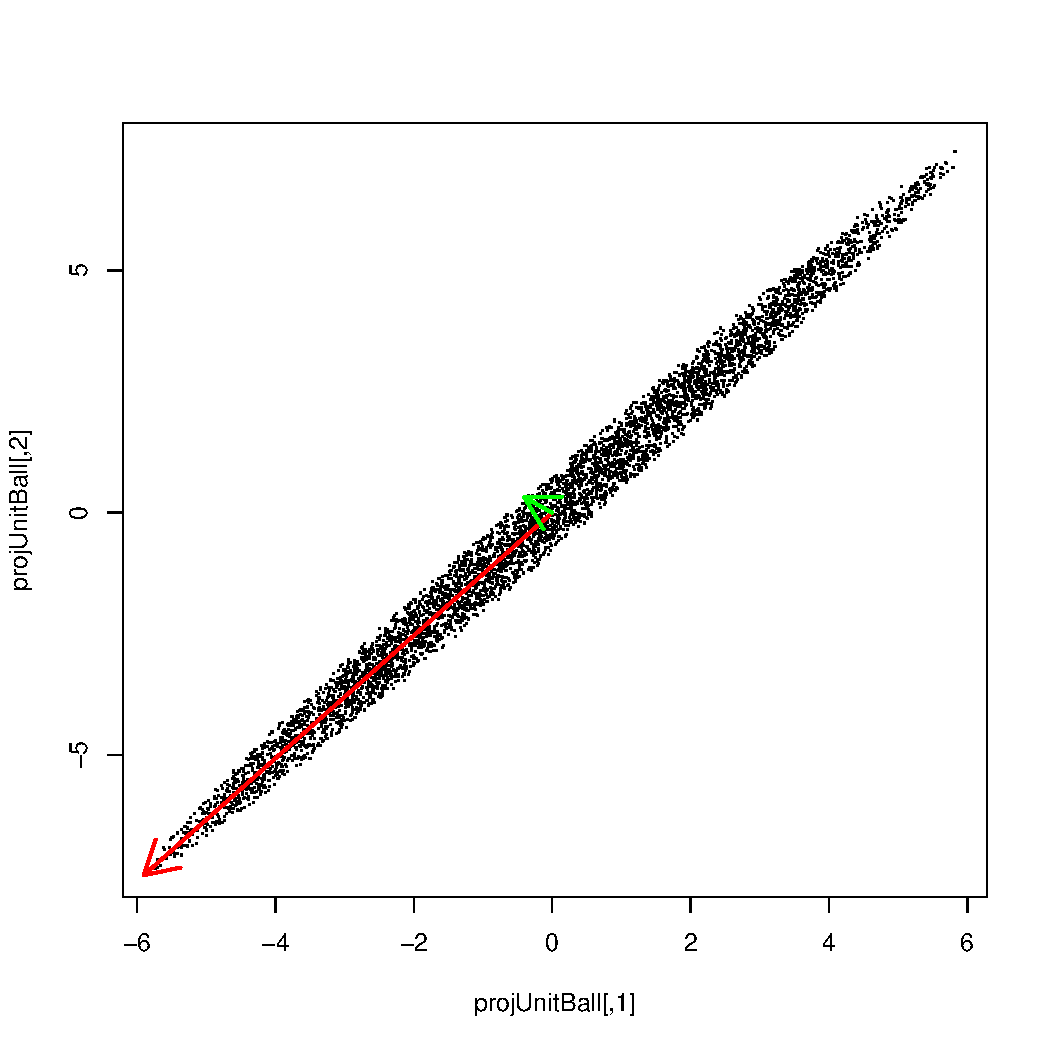
\includegraphics[width=3.5in]{img/fig05.pdf}
\end{center}

\end{frame}

%%%%%%%%%%%%%%%%%%%%%%%%%%%%%%%%%%%%%%%%%%%%%%%%%%%
\begin{frame}[fragile] \frametitle{}

Now consider the following quantity for a full rank matrix $A$:
\begin{align*}
\frac{|| A\delta ||_2}{||\delta||_2}
\end{align*}
\pause Let $\delta = \sum_i \alpha_i v_i$. Then:
\begin{align*}
\frac{|| A\delta ||_2}{||\delta||_2}
  &= \sqrt{\frac{\sum_i \sigma_i^2 \alpha_i^2 v_i^2}{\sum_i \alpha_i^2 v_i^2}}
\end{align*}
\pause We can see that the minimum occurs when $\delta$ is equal to $v_{\text{min}(n,m)}$.

\pause Likewise, the maximum occurs when $\delta$ is equal to $v_1$.

\end{frame}

%%%%%%%%%%%%%%%%%%%%%%%%%%%%%%%%%%%%%%%%%%%%%%%%%%%
\begin{frame}[fragile] \frametitle{}

So, we have the following inequality for all $\delta \neq 0$:
\begin{align*}
\sigma_{\text{min}} \leq \left\{\frac{|| A\delta ||_2}{||\delta||_2}\right\} \leq \sigma_{\text{max}}
\end{align*}
For the singular values $\sigma_{\text{min}}$ and $\sigma_{\text{max}}$.

\end{frame}

%%%%%%%%%%%%%%%%%%%%%%%%%%%%%%%%%%%%%%%%%%%%%%%%%%%
\begin{frame}[fragile] \frametitle{}

Finally, notice that the inner product can be written compactly in terms of
the singular values:
\begin{align*}
A^t A &= V \Sigma^t U^t U \Sigma V^t \\
&=  V \Sigma^2 V^t
\end{align*}
\pause This just the eigenvalue decomposition of the matrix $A^t A$. Notice
that the eigenvalues of $A^t A$ are the squares of the singular values of
$A$.

\end{frame}

%%%%%%%%%%%%%%%%%%%%%%%%%%%%%%%%%%%%%%%%%%%%%%%%%%%
\begin{frame}[fragile] \frametitle{}

\textbf{Back to linear models}

In a linear model, we only observe $X \beta$, rather than $\beta$ itself.
We have already seen that numerical problems can lead to multiple solutions
for which the $X\beta$'s is very similar but the regression vectors $\beta$
are quite different.

\end{frame}


%%%%%%%%%%%%%%%%%%%%%%%%%%%%%%%%%%%%%%%%%%%%%%%%%%%
\begin{frame}[fragile] \frametitle{}

Say that we have an error (or noise) $\Delta$ in the term $\beta$.
Formally, we  wish to control the ratio of the relative error in
estimation to that of projection: \pause
\begin{align*}
\frac{\text{rel. error estimation}}{\text{rel. error projection}}
 &= \frac{|| \beta + \Delta ||_2 / || \beta ||_2}{|| X(\beta + \Delta) ||_2 / || X\beta ||_2}
 < \epsilon
\end{align*}
\pause So we do not want large changes in $\Delta$ to yield relatively
small changes in the prediction space $X\beta$.

\end{frame}

%%%%%%%%%%%%%%%%%%%%%%%%%%%%%%%%%%%%%%%%%%%%%%%%%%%
\begin{frame}[fragile] \frametitle{}

Notice that we can re-arrange the equation as:
\begin{align*}
\frac{|| \beta + \Delta ||_2 / || X(\beta + \Delta) ||_2}{|| \beta ||_2 / || X\beta ||_2}
\end{align*}
And now we have an upper bound on the numerator and an lower bound on the
denominator via the singular values:
\begin{align*}
\frac{\text{rel. error estimation}}{\text{rel. error projection}} \leq \frac{\sigma_{max}}{\sigma_{min}}
\end{align*}
\pause This is called the \textit{condition number} of the matrix $A$, and was the
quantity R complained about last week when I tried to invert an ill-conditioned
matrix.

\end{frame}

%%%%%%%%%%%%%%%%%%%%%%%%%%%%%%%%%%%%%%%%%%%%%%%%%%%
\begin{frame}[fragile] \frametitle{}

The $\Delta$ in this equation could be (amongst other things)
numerical error, measurment error, or statistical noise. In any
case, badly conditions matrices $X$ make solving linear systems
difficult.

\end{frame}

%%%%%%%%%%%%%%%%%%%%%%%%%%%%%%%%%%%%%%%%%%%%%%%%%%%
\begin{frame}[fragile] \frametitle{}

\textbf{Mean squared error}

Completely switching topics for the moment, consider the mean
squared error (MSE) of an estimator $\widehat{\beta}$:\pause
\begin{align*}
\mathbb{E} || \beta - \widehat{\beta} ||_2^2
&= \mathbb{E} \sum_j (\beta_j - \widehat{\beta})^2\\
&= \sum_j \mathbb{E} (\beta_j - \widehat{\beta})^2\\
&= \sum_j \text{Var} (\widehat{\beta}_j) + \left[\mathbb{E} (\beta_j - \widehat{\beta}) \right]^2\\
&= \text{tr} (\text{Var}(\widehat{\beta})) + ||\text{Bias}(\widehat{\beta}) ||_2^2
\end{align*}
\pause This is the multivariate version of the version you (hopefully) saw in
introductory statistics.

\end{frame}

%%%%%%%%%%%%%%%%%%%%%%%%%%%%%%%%%%%%%%%%%%%%%%%%%%%
\begin{frame}[fragile] \frametitle{}

The mean squared error of the ordinary least squares estimator can be
calculated as follows, given the formula we derived for the variance
and the fact that it is unbiased:
\begin{align*}
\text{MSE} (\widehat{\beta}_{OLS})
  &= \text{tr} \left[ \sigma^2 (X^t X)^{-1} \right] \\
  &= \sigma^2 \text{tr} \left[(X^t X)^{-1} \right]
\end{align*}

\end{frame}

%%%%%%%%%%%%%%%%%%%%%%%%%%%%%%%%%%%%%%%%%%%%%%%%%%%
\begin{frame}[fragile] \frametitle{}

On the last homework, I ask you to look at an estimator which
has been shrunk towards zero by a factor of $\alpha$:
\begin{align*}
\mathbb{\widehat{\beta}}_\alpha &= \alpha \cdot \widehat{\beta}_{OLS}
\end{align*}
You then compared the mean squared error of this to the standard
ordinary least squares solution using a series of simulations.

\pause Let's calculate the mean squared error directly.

\end{frame}

%%%%%%%%%%%%%%%%%%%%%%%%%%%%%%%%%%%%%%%%%%%%%%%%%%%
\begin{frame}[fragile] \frametitle{}

We see quickly that:
\begin{align*}
\text{MSE} (\widehat{\beta}_{\alpha})
  &= \text{tr} (\text{Var}(\widehat{\beta}_{\alpha})) + ||\text{Bias}(\widehat{\beta}_{\alpha}) ||_2^2 \\
  &= \alpha^2 \sigma^2 \text{tr} \left[(X^t X)^{-1} \right] + (1-\alpha)^2 ||\beta||_2^2
\end{align*}
\pause What is the relationship between the optimal $\alpha$ and the quantities
$\sigma^2$ and $||\beta||_2^2$?

\end{frame}

%%%%%%%%%%%%%%%%%%%%%%%%%%%%%%%%%%%%%%%%%%%%%%%%%%%
\begin{frame}[fragile] \frametitle{}

\large
Sacrificing bias for a reduction in variance is, generally, a very
good idea, but we are not doing so in a very intelligent way here.

\end{frame}

%%%%%%%%%%%%%%%%%%%%%%%%%%%%%%%%%%%%%%%%%%%%%%%%%%%
\begin{frame}[fragile] \frametitle{}

What is the quantity $\text{tr} \left[(X^t X)^{-1} \right]$? \pause
Well, in terms of singular values we have:
\begin{align*}
\text{tr} \left[(X^t X)^{-1} \right]
&=\text{tr} \left[(V \Sigma^2 V^t)^{-1} \right] \\
&=\text{tr} \left[V \Sigma^{-2} V^t \right] \\
&=\text{tr} \left[\Sigma^{-2} V^t V \right] \\
&=\text{tr} \left[\Sigma^{-2} \right] \\
&=\sum_{i=1}^{r} \frac{1}{\sigma_i^2}
\end{align*}
\pause So a disproportionate amount of variance is coming from the
smallest singular values.

\pause \textbf{What if we could just shrink the variance in the
directions of the lowest singular values?}

\end{frame}

%%%%%%%%%%%%%%%%%%%%%%%%%%%%%%%%%%%%%%%%%%%%%%%%%%%
\begin{frame}[fragile] \frametitle{}

Two possible solutions:

(1) \textbf{Principal component regression} uses only the first
$k$ singular vectors of the data matrix $X$ in the regression
model.

(2) \textbf{Ridge regression} scales the ordinary least squares
solution by shrinking a small amount in the direction of the
largest singular values and a large amount in the direction of
the smallest singular values.

\end{frame}

%%%%%%%%%%%%%%%%%%%%%%%%%%%%%%%%%%%%%%%%%%%%%%%%%%%
\begin{frame}[fragile] \frametitle{}

\textbf{Summary of today's lecture}

\begin{enumerate}
\item Singular value decomposition can be applied to any real
matrix $A$ without regard to its shape or structure. \pause
\item Singular values are a generalization of eigenvalues.\pause
\item The ratio of the largest singular value to the smallest
singular value indicates how difficult it is to solve the
linear system $y = Ab$ by least squares. The quantity is called
the condition number of the matrix.\pause
\item The smallest singular value directions contribute a disproportionate
amount of variance in the estimation of the regression vector using
ordinary least squares.
\end{enumerate}

\end{frame}

\end{document}











